%%%%%%%%%%%%%%%%%%%%%%%%%%%%%%%%%%%%%%%%%
% Stylish Article
% LaTeX Template
% Version 2.2 (2020-10-22)
%
% This template has been downloaded from:
% http://www.LaTeXTemplates.com
%
% Original author:
% Mathias Legrand (legrand.mathias@gmail.com) 
% With extensive modifications by:
% Vel (vel@latextemplates.com)
%
% License:
% CC BY-NC-SA 3.0 (http://creativecommons.org/licenses/by-nc-sa/3.0/)
%
%%%%%%%%%%%%%%%%%%%%%%%%%%%%%%%%%%%%%%%%%

%----------------------------------------------------------------------------------------
%	PACKAGES AND OTHER DOCUMENT CONFIGURATIONS
%----------------------------------------------------------------------------------------

\documentclass[fleqn,11pt]{SelfArx} % Document font size and equations flushed left

\usepackage[spanish]{babel} % Specify a different language here - english by default

\usepackage{lipsum} % Required to insert dummy text. To be removed otherwise
\usepackage{tikz}
%\usepackage{newtxmath} % Cambia la fuente (pero mola)



\newcommand{\parentesis}[1]{\left( #1  \right)} 
\newcommand{\parciales}[2]{\frac{\partial #1}{\partial #2}}
\newcommand{\pparciales}[2]{\parentesis{\parciales{#1}{#2}}}
\newcommand{\ccorchetes}[1]{\left[ #1  \right]}
\newcommand{\D}{\mathrm{d}}
\newcommand{\derivadas}[2]{\frac{\D #1}{\D #2}}

\newcommand{\In}{\mathbf{I}}
\newcommand{\Jn}{\mathbf{J}}

\newcommand{\Rn}{\mathbf{R}}
\newcommand{\Ln}{\mathbf{L}}
\newcommand{\Un}{\mathbf{U}}
\newcommand{\Bn}{\mathbf{B}}
\newcommand{\Omegan}{\boldsymbol{\Omega}}


\newcommand{\rn}{\mathbf{r}}

\newcommand{\Ical}{\mathcal{I}}
\newcommand{\Ocal}{\mathcal{O}}
\newcommand{\Ucal}{\mathcal{U}}


%----------------------------------------------------------------------------------------
%	COLUMNS
%----------------------------------------------------------------------------------------

\setlength{\columnsep}{0.55cm} % Distance between the two columns of text
\setlength{\fboxrule}{0.75pt} % Width of the border around the abstract

%----------------------------------------------------------------------------------------
%	COLORS
%----------------------------------------------------------------------------------------

\definecolor{color1}{RGB}{0,0,90} % Color of the article title and sections
\definecolor{color2}{RGB}{0,20,20} % Color of the boxes behind the abstract and headings

\definecolor{darkgreen}{rgb}{0.15, 0.4, 0.0} % Valores de 0 a 1

\definecolor{naranja}{RGB}{255, 171, 0} % Valores de 0 a 1
\definecolor{morado}{RGB}{151, 0, 151} % Valores de 0 a 1

%----------------------------------------------------------------------------------------
%	HYPERLINKS
%----------------------------------------------------------------------------------------

\usepackage{hyperref} % Required for hyperlinks

\hypersetup{
	hidelinks,
	colorlinks,
	breaklinks=true,
	urlcolor=color2,
	citecolor=color1,
	linkcolor=color1,
	bookmarksopen=false,
	pdftitle={Title},
	pdfauthor={Author},
}

\usepackage[font=small, justification=centering]{caption}  % Configura las captions

%----------------------------------------------------------------------------------------
%	ARTICLE INFORMATION
%----------------------------------------------------------------------------------------

\JournalInfo{Trabajo voluntario} % Journal information
\Archive{Fisica nuclear y partículas} % Additional notes (e.g. copyright, DOI, review/research article)

\PaperTitle{Difusión elástica resonante} % Article title

\Authors{Daniel Vázquez Lago\textsuperscript{1}*} % Authors
\affiliation{\textsuperscript{1}\textit{Facultad de Física, Universidad Santiago de Compostela, Galicia, España}} % Author affiliation 
\affiliation{*\textbf{Correo del autor}: danielvazquezlago@gmail.com, daniel.vazquez.lago@rai.usc.es} % Corresponding author

\Keywords{Difusión elástica resonante, Resonancia, Formalismo R-Matricial, Difusión Elástica, Núcleo Compuesto, Reacción Directa, Breit-Wigner, Rsonancia, Canal, Ciclo CNO, Type I X-ray Buster, Escintilador, PPAC} % Keywords - if you don't want any simply remove all the text between the curly brackets
\newcommand{\keywordname}{Palabras clave} % Defines the keywords heading name

%----------------------------------------------------------------------------------------
%	ABSTRACT
%----------------------------------------------------------------------------------------

\Abstract{En este trabajo estudiaremos las difusiones elásticas resonantes y sus aplicaciones en el ámbito particular de la física nuclear, tratando de responder a las siguientes preguntas: ¿Qué es una difusión elástica resonante?¿Cómo se comporta la sección eficaz en una difusión elástica resonante?¿Cual es el interés de las dispersiones elásticas resonantes?¿Qué las diferencia de una difusión inelástica? Tratando de responder a estas preguntas estudiaremos entonces diferentes modelos matemáticos que nos permiten introducir las secciones eficaces y diferentes aplicaciones para ver cual es la potencia e interés de las difusiones elásticas resonantes.}

%----------------------------------------------------------------------------------------

\begin{document}

\maketitle % Output the title and abstract box

\tableofcontents % Output the contents section

\thispagestyle{empty} % Removes page numbering from the first page


\setlength{\parskip}{1.5mm} % Cambia el espacio entre párrafos


%----------------------------------------------------------------------------------------
%	ARTICLE CONTENTS
%----------------------------------------------------------------------------------------

\section{Introducción}

Para tratar de entender un poco el fenómeno de la difusión elástica resonante primero tenemos que tratar un poco la historia de las difusiones. Las difusiones o colisiones entre partículas se empezaron a estudiar a principios del siglo XX por Marsden, Geiger, Rutherford, estudiando como se comportaba un haz partículas $\alpha$ al colisionar con diferentes planchas de metal, observando que parte de las partículas interaccionaban fuertemente con el metal cuando incidía con ángulos más allá de los 90$^\circ$. El propósito de esta investigación era dilucidar como eran los átomos, conocer su estructura interna y forma. De hecho, de estos experimentos Rutherford dedujo que los núcleos estaban formados por un núcleo cargado positivamente y un halo de partículas poco pesadas cargadas negativamente orbitando a su alrededor, que denominó electrones. Mas tarde Darwin derivó una fórmula (usando la mecánica clásica) que describía la sección eficaz de la difusión elástica de Rutherford, que es el nombre que se le da a las difusiones elásticas entre partículas cargadas. Esta viene dada por \cite{FNyP}:

\begin{equation}
	\parentesis{\derivadas{\sigma(\theta)}{\Omega}}_{\text{Rutherford}} = \parentesis{\frac{1}{ 4 \pi \epsilon_0}}^2 \frac{Z_1Z_2 e^2}{(4E)^2\sin^4 (\theta/2)}
\end{equation}
donde $Z_2$ es la carga el haz incidente y $E$ su energía. Aunque esta sección eficaz se dedujo usando la mecánica clásica, también es posible deducirla a través de la mecánica cuántica (y se obtiene la misma fórmula, siempre que no se tenga en cuenta el espín y correcciones relativistas). Sin embargo pocos años después en el estudio de otras difusiones se obtuvieron secciones eficaces con anomalías. Estas anomalías se manifestaron generalmente en forma de picos para energías concretas, picos llamados \textbf{resonancias}, y como eran resonancias en la difusión elástica se le llamo a este fenómeno \textbf{difusión elástica resonante}.  

Tras el descubrimiento del neutrón (1932) se comenzó a estudiar también la dispersión de estos ya que al no tener carga y por tanto no estar sometidas a la dispersión de Rutherford los neutrones deberían de ser capaces de penetrar directamente en el núcleo del átomo, incluso a energías bajas. Al igual que con los protones, la sección eficaz caía con la energía y también mostraba picos súbitos, tal y como podemos ver en la siguiente imagen:

\begin{figure}[h!] \centering
	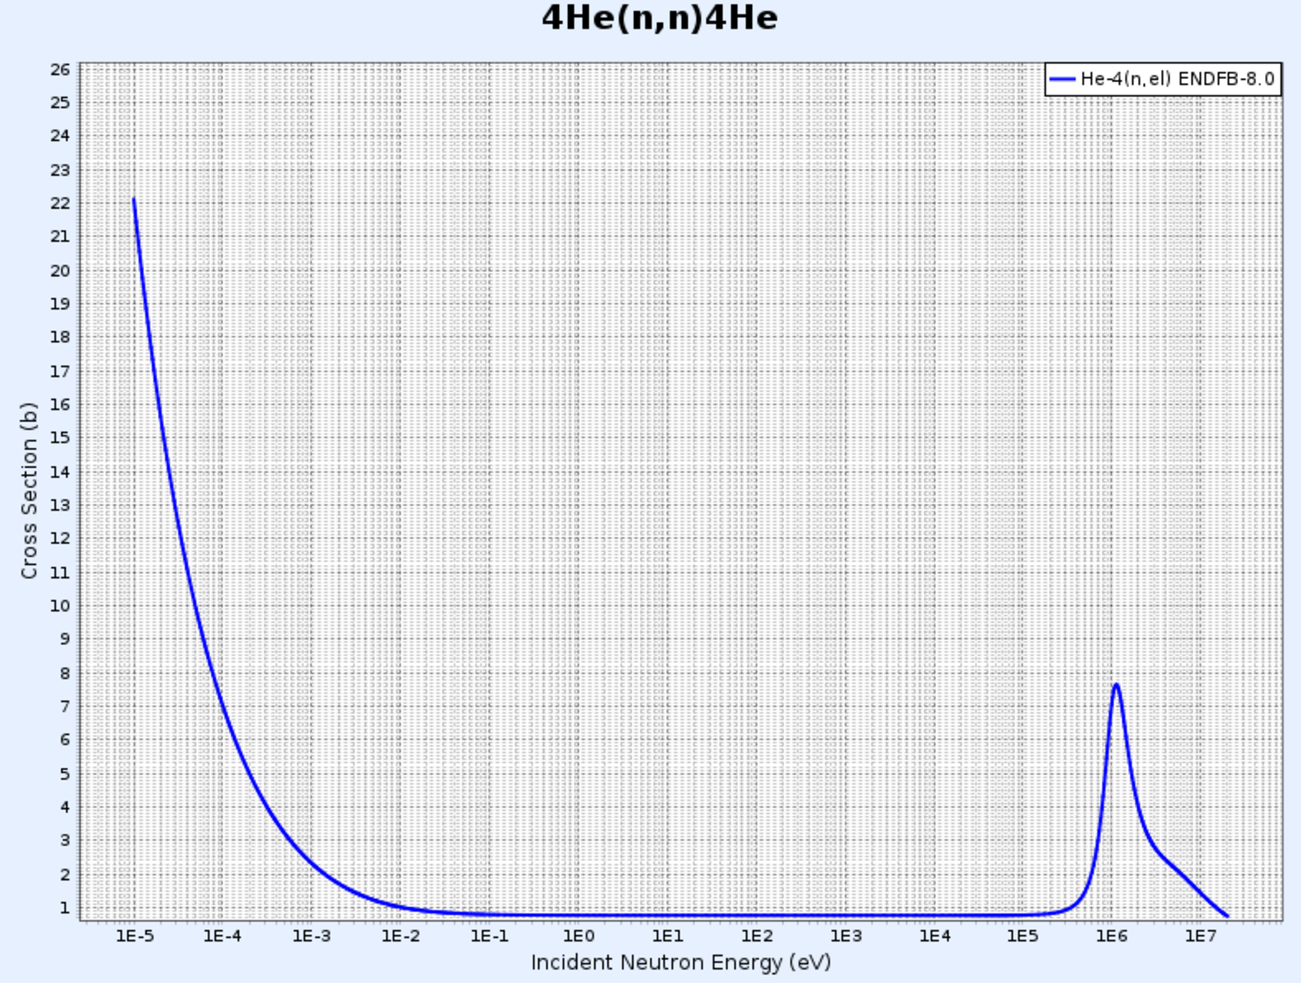
\includegraphics[width=0.5\textwidth]{He.png}
	\caption{Sección eficaz dispersión elástica $^4$He(n,n)$^4$He.}
\end{figure}
Existe una similitud entre uno y otro fenómeno, y la similitud fue resuelta en 1936 cuando Niels Bohr propuso el modelo del \textbf{núcleo compuesto}, en el que se considera que la reacción tiene lugar a través de un estado nuclear intermedio o núcleo compuesto (modelo basado en la gota líquida) en el que los nucleones llegan a compartir toda la energía. Esto explicaría que los picos se formaran en determinadas energías, ya que los estados compuestos solo se formarían a energías muy concretas al ser estados metaestables o inestables (ya que en el caso de ser estables tendríamos que la reacción sería profundamente inelástica). Es más, esto también explicaría porque algunas dispersiones elásticas e inelásticas (y las diferentes dispersiones inelásticas) con las mismas partículas incidentes tienen los picos en las mismas energías: la formación del estado compuesto es la misma, la única diferencia viene dada por el canal de salida, tal y como podemos ver en las imagenes \ref{Fig:02} y \ref{Fig:03}.

\begin{figure}[h!] \centering
	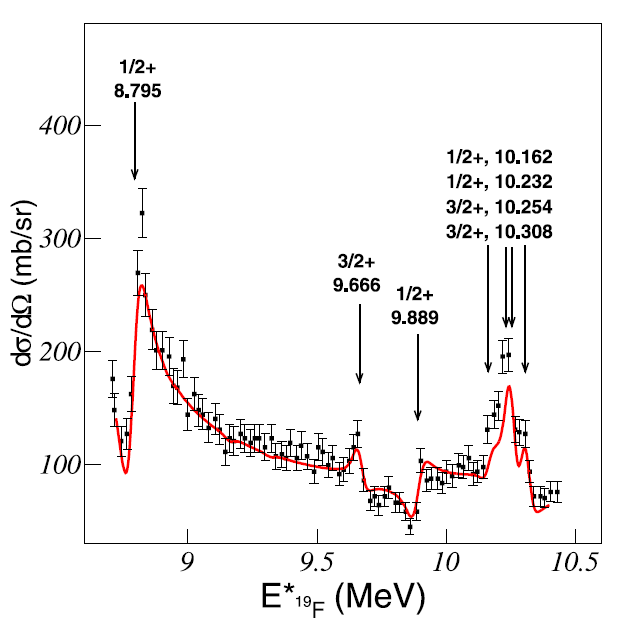
\includegraphics[width=0.45\textwidth]{01.png}
	\caption{Sección eficaz de la difusión elástica $^{19}$F(p,p)$^{19}$F a través de distintas resonancias del $^{20}$Ne. Imagen de \cite{USC}.}
	\label{Fig:02}
\end{figure}
\begin{figure}[h!] \centering
	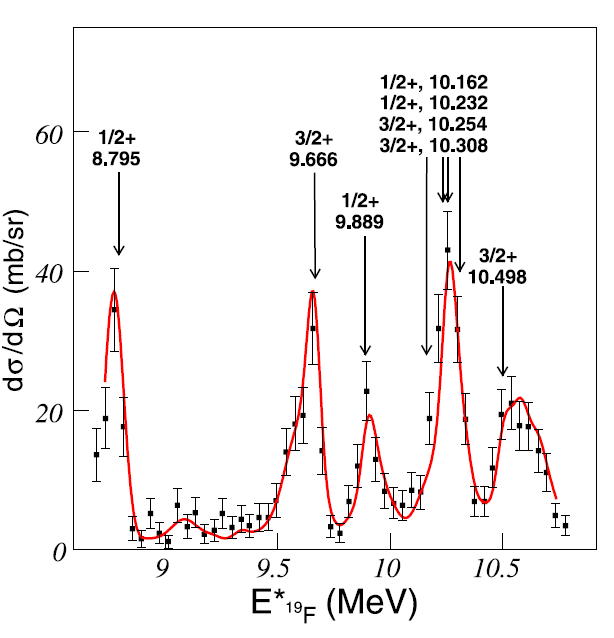
\includegraphics[width=0.45\textwidth]{02.png}
	\caption{Sección eficaz de la difusión inelástia $^{19}$F(p,$\alpha$)$^{16}$O a través de distintas resonancias del $^{20}$Ne. Imagen de \cite{USC}.}
	\label{Fig:03}
\end{figure}

Más tarde (Butler, 1950) se descubrieron las \textbf{reacciones directas}, que son un tipo de reacción nuclear (igual que las del núcleo compuesto) en las que los núcleos no llegan a formar un núcleo compuesto, interaccionando directamente. Estas reacciones están entre las reacciones elásticas clásicas y las reacciones por núcleo compuesto, ya que no se forma un núcleo compuesto pero es la probabilidad de que pueda ocurrir la que hace que aumente súbitamente la sección eficaz. 

Una vez tenemos esto podemos decir que existen dos \textit{fenómenos simultáneos} que intervienen para formar la \textbf{difusión elástica resonante}: la difusión elástica (figura \ref{Fig:04}) (en el caso de partículas cargadas la dispersión de Rutherford) y la difusión elástica a través de la  formación de un núcleo compuesto/reacción directa (o una mezcla de ambos, aunque la mayoría suele preponderar el primer tipo de reacción) (figura \ref{Fig:05}). Como sabemos en la física cuántica que estos dos fenómenos operen simultáneamente significa que la sección eficaz total no es la suma de ambas, ya que existe interferencia entre ambos fenómenos. La teoría que trate de describir los fenómenos tendrá que tener en cuenta la posible interferencia entre los fenómenos.

\begin{figure}[h!] \centering
	\begin{tikzpicture}[thick,scale=0.6]
		% 1a parte
		\node at (-3.6,-1.1) [circle,draw=red!50,fill=red!20] {};
		
		\node at (-3.6,1.1) [circle,draw=darkgreen!50,fill=darkgreen!20] {};
		
		\node (1) at (-3.5,1) {};
		\node (2) at (-3.5,-1) {};
		
		\draw[arrows={->},ultra thick,darkgreen!90] (1.east)--(0.0,0.2)  ;
		\draw[arrows={->},ultra thick,red] (2.east)--(0.0,-0.2)  ;
		
		\node (1) at (-3.6,1.9) {$\alpha_1$};
		\node (2) at (-3.6,-1.9) {$\alpha_2$};
		
		
		% 2a parte
		\node at (3.8,-1.1) [circle,draw=red!50,fill=red!20] {};
		
		\node at (3.8,1.1) [circle,draw=darkgreen!50,fill=darkgreen!20] {};
		
		\node (1) at (3.7,1) {};
		\node (2) at (3.7,-1) {};
		
		\draw[arrows={->},ultra thick,darkgreen!90] (0.4,0.2)--(1.west)  ;
		\draw[arrows={->},ultra thick,red](0.4,-0.2)-- (2.west)  ;
		\node (1) at (3.8,1.9) {$\alpha_1$};
		\node (2) at (3.8,-1.9) {$\alpha_2$};
		
	\end{tikzpicture}
	\caption{Dispersión elástica 1+2$\rightarrow$1+2.}
	\label{Fig:04}
\end{figure}


\begin{figure}[h!] \centering
	\begin{tikzpicture}[thick,scale=0.6]
		
		% 1a parte
		\node at (-3.6,-1.1) [circle,draw=red!50,fill=red!20] {};
		
		\node at (-3.6,1.1) [circle,draw=darkgreen!50,fill=darkgreen!20] {};
		
		\node (1) at (-3.5,1) {};
		\node (2) at (-3.5,-1) {};
		
		\draw[arrows={->},ultra thick,darkgreen!90] (1.east)--(0.0,0.2)  ;
		\draw[arrows={->},ultra thick,red] (2.east)--(0.0,-0.2)  ;
		
		\node (1) at (-3.6,1.9) {$\alpha_1$};
		\node (2) at (-3.6,-1.9) {$\alpha_2$};
		
		% 2a parte
		
		\node (2) at (0.5,-0.95) {$\alpha_3$};
		\node at (0.5,0) [circle,draw=blue!70,fill=blue!40] {};
		
		% 3a parte
		\node at (4.6,-1.1) [circle,draw=red!50,fill=red!20] {};
		
		\node at (4.6,1.1) [circle,draw=darkgreen!50,fill=darkgreen!20] {};
		
		\node (1) at (4.5,1) {};
		\node (2) at (4.5,-1) {};
		
		\draw[arrows={->},ultra thick,darkgreen!90] (1.0,0.2)--(1.west)  ;
		\draw[arrows={->},ultra thick,red](1.0,-0.2)-- (2.west)  ;
		\node (1) at (4.6,1.9) {$\alpha_1$};
		\node (2) at (4.6,-1.9) {$\alpha_2$};
		
		
	\end{tikzpicture}
	\caption{Dispersión elástica por formación del núcleo compuesto 1+2 $\rightarrow$ 3 $\rightarrow$ 1+2.}
	\label{Fig:05}
\end{figure}

\section{Formalismo R-Matricial}

Al igual que a principios de siglo XX, las difusiones son interesantes porque nos permiten obtener información de los núcleos atómicos. Sin embargo para esto necesitamos una teoría que sea capaz de describir de manera adecuada las reacciones nucleares y las difusiones particularmente, de tal modo que podamos relacionar de alguna las piezas de información conocidas en el laboratorio (sección eficaz diferencial, naturaleza partículas emitidas e incidentes, momentos y energías de las partículas incidentes y emitidas...) con parámetros o información del núcleo (como podría ser energías de excitación, espín, forma...). Una de las teorías más extendidas es la del formalismo R-Matricial, del que veremos un poco su historia para entenderla un poco mejor, a través del \cite{Biblia} pag. 259-264.

\subsection{Historia del formalismo R-Matricial}

Cuando Bohr propuso el modelo del núcleo atómico no existía un formalismo riguroso en la mecánica cuántica que pudiera describirlo cuantitativamente. La única teoría que existía era la \textit{teoría de Weisskopf-Wigner}, que describía la absorción resonante y posterior emisión de radiación electromagnética por un sistema atómico. Breit y Wigner trataron de adaptar esta teoría a las reacciones nucleares, resultando en la \textbf{ecuación de Briet-Wigner} que hoy conocemos para un canal de entrada $c$ y uno de salida $c'$ \cite{FNyP} 

\begin{equation}
	\sigma_{cc'} = \frac{\pi}{k^2} g_J \parentesis{\frac{\Gamma_{c} \Gamma_{c'}}{(E-E_r)^2 + \Gamma^2 / 4}}
\end{equation}
siendo $g_J$ el factor estadístico de espín que más adelante explicaremos, $\Gamma$ la anchura de la resonancia, $E_r$ la energía de la resonancia, $\Gamma_{c}$ la anchura parcial del canal de entrada y $\Gamma_{c'}$ la anchura parcial del canal de salida. Aunque el tratamiento perturbativo en reacciones nucleares no es del todo correcto, las expresiones de sección eficaz obtenidas por la fórmula coincidían bastante bien con los valores experimentales (en su dependencia con la energía claro está) siempre y cuando claro la resonancia fuera aislada. Y, aunque esta fórmula se ajuste bien a los datos experimentales, hay que decir que no es una buena fórmula en el sentido más físico, ya que está adaptando una teoría que sirve para un fenómeno muy diferente al que se quiere tratar (la resonancia de Weisskopf-Wigner se debe a una fuerza débil como es la electromagnética, mientras que las reacciones nucleares tratan fuerzas fuertes).

Wigner y Eisenbud, inspirados por otras teorías como la de Kapur y Peierls, introdujeron lo que hoy llamamos \textbf{teoría de la matriz-R} o \textbf{formalismo R-Matricial}, una teoría que sirve para describir ``cualquier tipo'' de reacción nuclear, y no solo aquellas mediadas por el núcleo compuesto, sino incluso las reacciones directas, aunque su especialidad sigue siendo describir las reacciones por núcleo compuesto. El gran avance de está teoría respecto a otras hechas es que la dependencia energética se hace de manera más explícita, lo que la hace más fácil de aplicar y entender.


\subsection{Limitaciones del formalismo R-Matricial}

El formalismo R-Matricial tiene una serie de limitaciones, como es el caso de las reacciones nucleares que impliquen núcleos con muchos nucleones, ya que el formalismo R-matricial trata con estados estáticos. Otras limitaciones son:

\begin{itemize}
	\item Aplicabilidad de la física no relativista y por tanto de la ecuación de Schrödinger.
	\item Ausencia de todo fenómeno que implique que el núcleo compuesto se divida en 3 núcleos/partículas. Esta es la más restrictiva de todas las limitaciones.
	\item Ausencia de todo fenómeno que genere partículas o las destruya, limitando por ejemplo la teoria a reacciones que no produzcan fotones, aunque mediante teoría de perturbaciones se puede modificar \cite{Biblia} pag. 
	\item La existencia de una distancia $a$ a partir la cual ya no haya interacciones entre potenciales no centrales. 
\end{itemize}




\subsection{Teoría del formalismo R-Matricial}

La idea detrás del formalismo R-Matricial es que existen dos regiones del espacio diferenciadas por una distancia particular $a$ en las que hay dos funciones de onda con diferente forma analítica.  En general $a$ se toma como el tamaño del núcleo compuesto $r=R_0A^{1/3}$, aunque recientes investigaciones recomiendan otro tipo de formulación. La región externa es solución de la ecuación de Schrödinger para un sistema de dos partículas $\alpha_1$ y $\alpha_2$, que usando combinaciones lineales se puede escribir como una función de ondas para la masa reducida. En ese caso la solución es bien sencilla, ya que el potencial para $r>a$ deben ser potenciales de largo alcance como puede ser el potencial de Coulomb si las partículas están cargadas o cero si por ejemplo estamos en reacciones en las que intervienen neutrones. De este modo podremos expresar la función de onda de la región externa como un producto de la función de espín y una combinación lineal de funciones de onda entrantes ($\Ical_c$) y salientes ($\Ocal_c$). La relación entre los coeficientes entrantes $I_c$ y salientes $O_c$ determinan por completo la sección eficaz.

La función de onda interna $r<a$ se expresará como una combinación lineal de varias funciones de onda considerados autoestados de la función global y el hamiltoniano. Hay que recordar que debido a la conservación de la paridad y del momento angular estas funciones de onda tienen limitado su momento angular y espín a unos concretos que dependen de las partículas entrantes.  

Lo que relaciona la función de onda interna y la función de onda externa es la condición de que la función de ondas global debe ser continua en la frontera $r=a$. Entonces en función de la onda interna evaluada exclusivamente en la superficie (consecuentemente no nos importa la forma que tenga dentro, eliminando toda posibilidad de comprender la dinámica de los nucleones) determinará la relación entre los coeficientes $I_c$ y $O_c$, y por tanto la sección eficaz. 

Vemos entonces que el formalismo R-matricial es bidireccional: de conocer la sección eficaz y otros valores experimentales podríamos deducir la relación de los coeficientes de entrada y salida y por tanto deducir los autovalores de las autofunciones en la superficie $r=a$, o, por el contrario, podemos suponer un potencial nuclear para deducir las funciones de onda internas de tal modo que podamos calcular la relación entre $I_c$ y $O_c$ para luego obtener la sección eficaz para este modelo. Un ejemplo muy interesante es el realizado por Francois de Oliveria Santos en \cite{Ressonant-Scattering-Elastic}, en el que supone como potencial un pozo y difusión de partículas sin espín y neutras. Obtiene así una expresión como la siguiente

\begin{equation}
	\sigma (E) = \frac{\pi}{k^2} \left| 2 \sin (ka)e^{ika} - \frac{\Gamma}{(E_\lambda - E) - i \frac{\Gamma}{2}} \right|^2
\end{equation}
que contiene términos de la difusión elástica por esfera dura (primer término) y términos de Briet-Winger (segundo término). Al tener el cuadrado de la suma también aparece términos de interferncia entre ambos términos.

Relacionar algebraicamente los estados internos y la sección eficaz puede ser realmente difícil, por eso se suelen introducir cantidades intermedias, como lo es la matriz $\Rn$ que nombra esta teoría y que representa las interacciones internas que ocurren en $a<r$ o las matrices $\Ln$ y $\Omegan$, y entender el significado de estos todavía puede llegar a ser más complicado. Para poder entender un poco más la potencial real de esta teoría veamos que datos podemos obtener a partir de los datos experimentales:

\begin{itemize}
\item Podemos obtener las energías de excitación de los estados del núcleo compuesto.
\item Debido a los fenómenos de interferencia que incluye el formalismo R-Matricial también nos permite obtener valores de los diferentes estados de espín, como se ha hecho a través de las reacciones $^{1}$H($^{18}$F,p)$^{18}$F y $^{18}$F(p,$\alpha$)$^{15}$O obteniendo el espín de estados excitados del $^{19}$Ne con interés en el estudio de mecanismos astrofísicos de novas \cite{18Fp}.
\item También se puede usar los valores de la sección eficaz para diferentes angulos para obtener los espines.
\end{itemize}

\begin{figure}[h!] \centering
	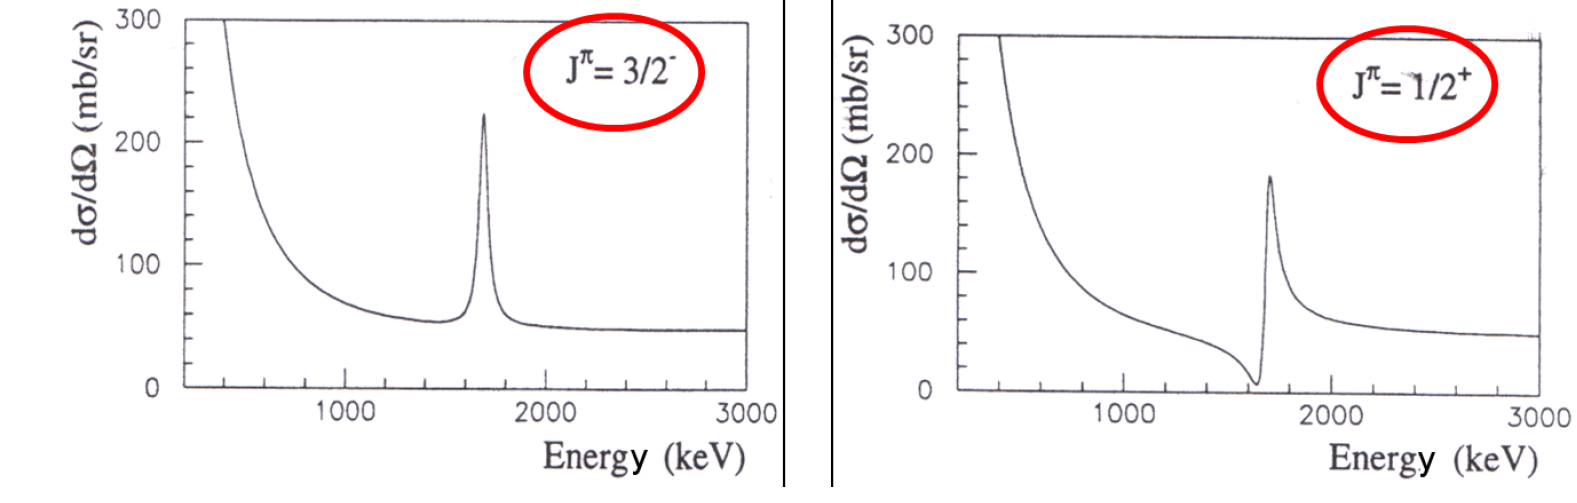
\includegraphics[width=0.45\textwidth]{Espines.png}
	\caption{Secciones eficaces para diferentes estados excitados del $^{13}N$ obtenidos a través la reacción elástica p+$^{12}$C \cite{Ressonant-Scattering-Elastic}.}
	\label{Fig:06}
\end{figure}

Por eso en general se suelen hacer aproximaciones, como puede ser la aproximación a una resonancia aislada, de la que se obtiene la ecuación de Briet-Wigner (en la primera aproximación del caso más sencillo, de tener en cuenta más términos en la ecuación la ecuación difiere cada vez más). Cabe destacar que a diferencia de esta ecuación el formalismo R-Matricial es mas potente que esta última, ya que también permite obtener la sección eficaz en términos de anchuras y energías de resonancias para resonancias no aisladas, así como la interferencia entre diferentes resonancias aisladas. En líneas generales: es una teoría mucho que nos permite adaptarnos a una gran cantidad de posibilidades, por lo que se ajusta muy bien a prácticamente cualquier curva experimental en la que medie el mecanismo del núcleo compuesto (excepto para casos con partículas con muchos nucleones).

\subsection{Canales y factor de espín}

Como hemos visto el formalismo matricial exige entonces un mínimo conocimiento, como pudiera ser el espín o momento, de las partículas incidentes en la reacción implicada, ya que determinan la función de ondas global. En general este último es difícil de conocer ya que las partículas incidentes suelen venir expresasdas como funciones de ondas planas o casi-planas que contienen infinitos momentos angulares. Por eso es necesario hablar de canales y espines.

Definimos como \textbf{canal de entrada} como al conjunto de de números cuánticos necesarios para describir la función de ondas parcial entrante, que en este caso son qué tipo de partículas denotadas por  $\alpha_1$ y $\alpha_2$, los espines $I_{\alpha_1}$ y $I_{\alpha_2}$ y las posibles excitaciones de las partículas (denotado por $\alpha$). Necesitamos 4 números para describir correctamente los espines de las partículas de entrada, que son el momento angular orbital total $\ell$, el momento espín total $s$, el momento angular total $J$ y el momento angular proyectado en el eje $z$ $m_J$. Así tenemos que
\begin{equation}
	c = \left\lbrace \alpha,\ell,s,J,m_j \right\rbrace
\end{equation}
De la misma manera describimos el canal de salida $c'$
\begin{equation}
	c' = \left\lbrace \alpha',\ell',s',J',m_j' \right\rbrace
\end{equation}
Lógicamente la conservación del momento angular total y de la paridad obliga a que ciertos canales de salida sean inviables, aunque si sean energéticamente posibles. La conservación del momento angular total nos dice que
\begin{equation}
	\Jn = \In_{\alpha_1}+\In_{\alpha_2}+\ell =  \In_{\alpha_1'}+\In_{\alpha_2'}+\ell' 
\end{equation}
y la paridad nos obliga a que:
\begin{equation}
	\pi = \pi_{\alpha_1}+\pi_{\alpha_2}+(-1)^{\ell} =  \pi_{\alpha_1'}+ \pi_{\alpha_2'} +(-1)^{\ell'} 
\end{equation}
La importancia de la conservación de momento angular y paridad es capital, ya que este introduce un factor estadístico ya que el \textit{número de combinaciones totales} entre $I_{\alpha_1}, I_{\alpha_2}$ y $\ell$ es $(2I_{\alpha_1}+1)(2I_{\alpha_2}+1)(2\ell+1)$, mientras que el \textit{número de combinaciones posibles} (debido a esta conservación) es $2J+1$. Esta es la razón por la cual las secciones eficaces dependen del momento angular total $J$ para un $\ell$ dado., y por tanto el \textbf{factor estadístico} $g_c(J)$
\begin{equation}
	g_c(J)=\frac{2J+1}{(2I_{\alpha_1}+1)(2I_{\alpha_2}+1)}
\end{equation}
debe ser tenido en cuenta. Esta es una de las correcciones que se suele aplicar a la ecuación de Briet-Wegner.

%\subsection{Sección de eficaz en el caso de una resonancia aislada y comparación con Breit-Wigner}

\section{¿Por qué las difusiones elásticas resonantes?}

Como hemos explicado el formalismo R-Matricial nos permite obtener información de las propiedades del núcleo, como pueden ser energías de resonancia, anchuras de resonancia, espín de los estados resonantes... Sin embargo el formalismo R-Matricial es tan bueno describiendo difusiones elásticas como difusiones inelásticas, y a partir de ambas se debería poder obtener el mismo de información siempre que el canal de entrada sea el mismo. 

Lo que hace interesante a las difusiones elásticas es la sencillez que tiene su aplicabilidad en la física experimental. Algunas de sus características son las siguientes:

\begin{itemize}
	\item En general las secciones eficaces de las difusiones elásticas son más grandes que las de las difusiones inelásticas, lo que hace que obtener datos sea mas fácil (y por ende tenga menos <<error>>). Recordemos que una mayor sección eficaz implica un mayor \textit{branching ratio} y por tanto mayor importancia relativa respecto a otras reacciones con el mismo canal de entrada. 
	\item A diferencia de algunas colisiones inelásticas, que pueden producir estados no ligados o excitados que decaigan rápidamente eliminando la información de la reacción de interés, en las difusiones elásticas conocemos perfectamente las partículas involucradas (estados de espín, estados excitados, masas...) por lo que obtener información es más sencilla. 
\end{itemize}
A pesar de todos suele ser necesario estudios simultáneos de difusiones elásticas e inelásticas para obtener parámetros. Uno de estos ejemplos puede ser el estudio de las reacciones $^{1}$H($^{18}$F,p)$^{18}$F y $^{18}$F(p,$\alpha$)$^{15}$O obteniendo datos sobre el $^{19}$Ne con interés en el estudio de mecanismos astrofísicos de novas \cite{18Fp} o el estudio de resonancias elásticas $\alpha$ y $\alpha$ simultáneamente con el $\alpha(\alpha,\gamma)^{8}$Be para obtener datos sobre el cluster de dos partículas $\alpha$ con interés astrofísico ya que dicho cluster es la puerta de entrada en la creación de átomos de $^{12}$C en estrellas en su fase de quema de He \cite{AlphaAlpha}. 


\section{Aplicación de la difusión elástica resonante: estudio de los estados resonantes protón del $^{18}$Ne}

En este apartado vamos a estudiar una de las múltiples aplicaciones de las difusiones elásticas resonantes, en este caso vamos a estudiar las propiedades de las resonancias de los protones en el átomo $^{18}$Ne a través de la difusión elástica $^{17}$F(p,p)$^{17}$F \cite{17Fp}.

\subsection{Interés del estado resonante protón del $^{18}$Ne }

Los estados exitados protón del $^{18}$Ne tienen un interés astrofísico particular debido a que aparece como núcleo compuesto en la reacción $^{14}$O($\alpha$,p)$^{17}$F, reacción que en los Type I X-ray burster puede desencadenar un paso a procesos $rp$ que produce núcleos ricos en protones (Tinanio, Vanadio...) \cite{Astrophysics}. Antes de continuar vamos a explicar un poco que es cada proceso que acabamos de mencionar

Los \textbf{Type I X-ray burster} es un fenómeno astrofísico asociado con estrellas binarias donde una estrella de neutrones acumula materia de una compañera, mientras que el \textbf{ciclo CNO} (Carbono-Nitrógeno-Oxígeno) es una cadena de reacciones termonucleares que convierte hidrógeno en helio utilizando elementos como carbono, nitrógeno y oxígeno  como catalizadores.

Conscuentemente conocer el comportamiento de la reacción  $^{14}$O($\alpha$,p)$^{17}$F permitiría entender mucho mejor este tipo de clusters y la creación de elementos pesados, lo cual implica que debemos saber cuales son sus energías de resonancia, formación etc, ergo necesitamos conocer el mecanismo de resonancia a través del núcleo compuesto $^{18}$Ne.
	
\subsection{Experimento}

Para obtener la sección eficaz necesitamos conocer la energía del haz incidente (para así hacer un estudio en función de la energía); una proporción alta de las partículas de interés en el haz, en nuestro caso $^{17}$F (para obtener un número de datos extenso sin interferencia de otras reacciones nucleares, disminuyendo el ruido); algún tipo de material que tenga propiedades que permitan una buena transmisión y dispersión de la energía generada por las colisiones, que contenga una cantidad de protones o átomos de H hidrógeno considerable (por la misma razón, para disminuir el ruido) y que de tener otro átomo que interaccione débilmente con el fluor (en nuestro caso $(CH_2)_n$ polietileno). Además necesitamos detectores de silicio en los ángulos de interés y algún otro tipo de detector para obtener resultados de la energía de las partículas en dicha dirección. Como veremos nuestro experimento requiere todas las exigencias que pedimos inicialmente.

El experimento descrito a continuación fue realizado en el instituto de investigación de iones pesados en Lanzhou (HIRFL). El experimento consta de los siguientes pasos. Primero se acelera $^{20}$Ne hasta los 70 MeV por nucleón por un ciclotrón que bombardea $^{9}$Be produciendo $^{17}$F$^{9+ }$,$^{16}$O$^{7+ }$,$^{18}$Ne$^{10+}$ entre otros iones. Este conjunto de productos tendrá que ser purificado (queremos obtener la mayor cantidad de iones $^{17}$F$^{9+ }$ posibles ya que es el haz incidente de la reacción). 

A través de una plancha de aluminio de $313\mu$m se purifica la muestra y se reduce la energía del $^{17}$F$^{9+ }$, a través de dos planchas, una de silicio $323\mu$m y otra de aluminio $294\mu$m y un escintilador\footnote{Un escintilador es un material que emite luz visible o ultravioleta cuando es excitado por partículas ionizantes, como electrones, protones, rayos gamma, etc. Estos materiales se utilizan en detectores de radiación para convertir la energía de las partículas ionizantes en luz que puede ser detectada y medida.} de C$_9$H$_{10}$. Tras esto rendijas purifican el haz y reducen de nuevo el $\Delta p/p$ de las partículas hasta un ratio del $1\%$ máximo. Este camino se ilustra en la imagen \ref{Fig:07}. 

\begin{figure}[h!] \centering
	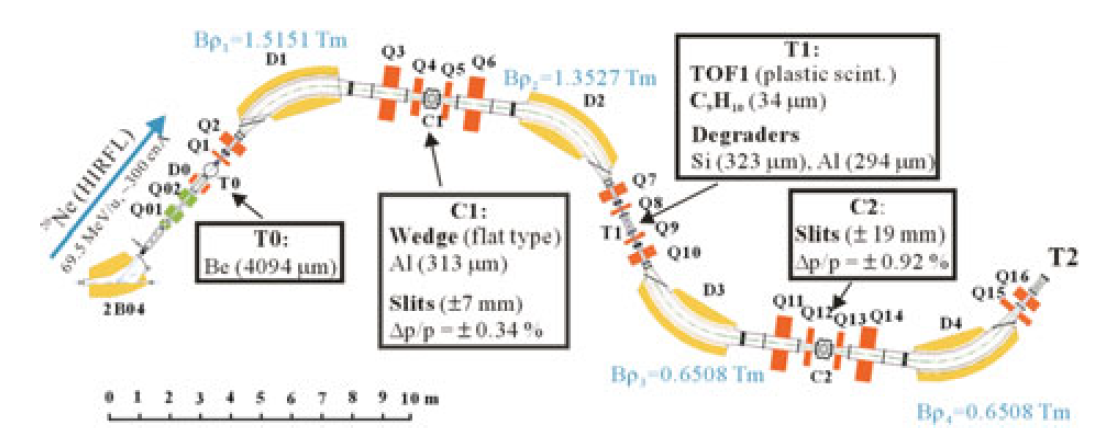
\includegraphics[width=0.5\textwidth]{exp1.png}
	\caption{Primera parte del experimento.}
	\label{Fig:07}
\end{figure}

En la siguiente parte tenemos otro escintor TOF2 como podemos ver en la imagen \ref{Fig:08} del que obtenemos la mezcla de partículas que componen el haz (figura \ref{Fig:09}) y un detector de silicio $280\mu$m para obtener la energía de las partículas. Ambos detectores se encuentran entre dos placas PPAC1 y PPAC2. Los PPACs \footnote{Contadores de Avalancha de Placas Paralelas son un tipo de detector de partículas que se utiliza en física nuclear y de partículas para detectar y medir partículas cargadas con alta precisión. Estos detectores son particularmente útiles en experimentos donde es importante determinar la posición de una partícula y su energía de manera eficiente y rápida} nos sirven para conocer la \textit{posición y ángulo de incidencia} del haz incidente extrapolando los resultados 2D de ambos PPACs. Cabe destacar que la resolución de estos últimos es de 1mm.


\begin{figure}[h!] \centering
	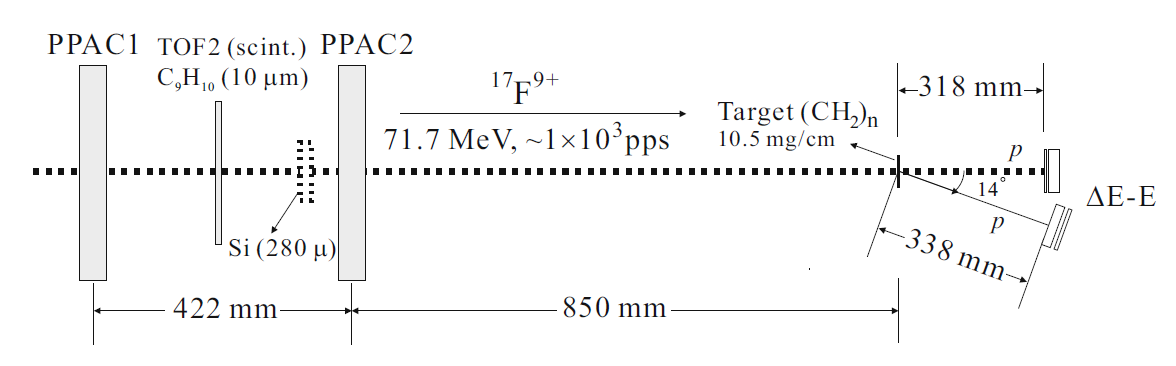
\includegraphics[width=0.5\textwidth]{exp2.png}
	\caption{Segunda parte del experimento.}	
	\label{Fig:08}
\end{figure}

\begin{figure}[h!] \centering
	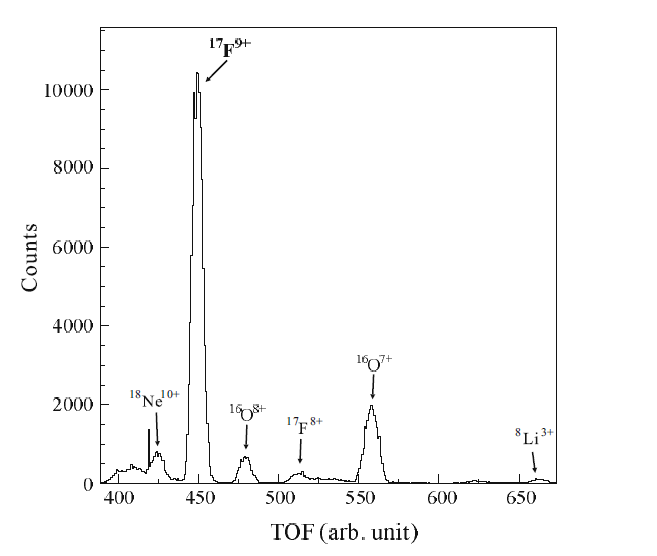
\includegraphics[width=0.5\textwidth]{counts.png}
	\caption{Número de cuentas de cada uno de los tipos de partículas creados en la reacción nuclear. Obtenido a través de los escintores y detectores de silicio.}
	\label{Fig:09}
\end{figure}

Una vez tenemos esto conocemos la dirección de incidencia en el objetivo $(CH_2)_n$ y la intensidad del haz $^{17}$F$^{+9}$ de $10^3$ partículas por segundo con una pureza del $50\%$. Tras esto 2 telescopios con un ángulo de laboratorio $\theta_{lab}\approx 0^\circ$ y $\theta_{lab}\approx 14^\circ$ que en el sistema centro de masas (sistema de referencia de interés) se traducen en ángulos  $\theta_{lab}\approx 175^\circ$ y $\theta_{lab}\approx 152^\circ$ respectivamente. El grosor del material objetivo será el suficiente como para que pierda energía de manera continua y obtengamos el espectro continuo de energías que queramos.
El valor de las energías de los protones emitidos en la reacción elástica se hace a través de detectores de silicio típicos que se pueden ver en \ref{Fig:09}.

\subsection{Análisis de datos}

Los datos obtenidos se representan en la figura \ref{Fig:10}, con un ajuste realizado a través de la R-Matriz. Como podemos ver el ajuste es ciertamente bastante correcto, y nos da como resultado las energías, anchuras, espines, momentos angulares e interferencia entre cada una de las posibles resonancias. Obtenemos entonces 3 resonancias aisladas (5.11, 7.34 y 7.71 MeV) y una resonancia doble en $\sim$ 7.1 MeV. El valor de los espines se obtiene viendo para que $\Jn$ se ajusta mejor a los datos, como podemos ver en la figura \ref{Fig:11}. También podemos ver que en la región de 1.6 MeV a 2.8 MeV de $E_{cm}$ no es posible obtener ningún tipo de información.

\begin{figure}[h!] \centering
	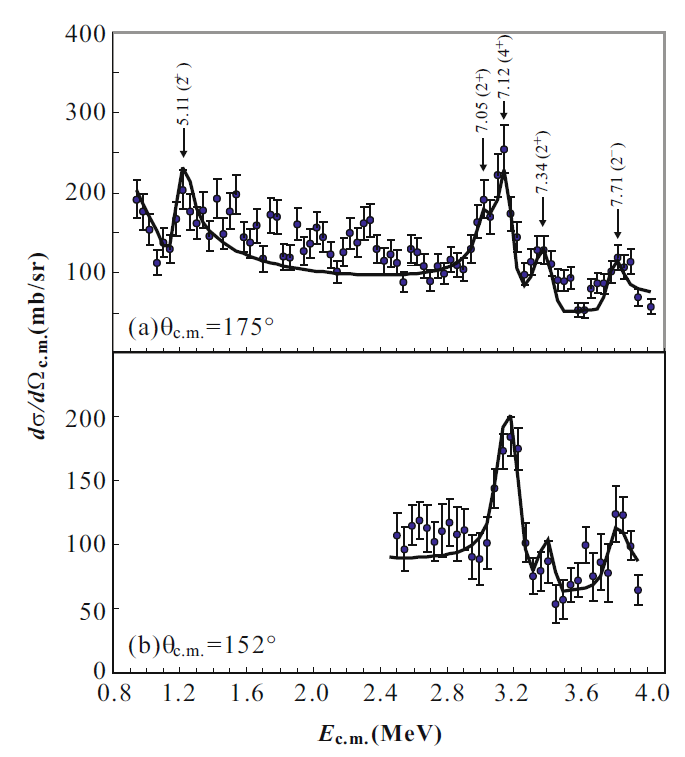
\includegraphics[width=0.5\textwidth]{diff cross.png}
	\caption{Secciones eficaces diferenciales en el centro de masa en la colisión $(CH_2)_n$ con partículas $^{17}$F a diferentes ángulos. Ajuste a través de la R-Matriz.}
	\label{Fig:10}
\end{figure}
\begin{figure}[h!] \centering
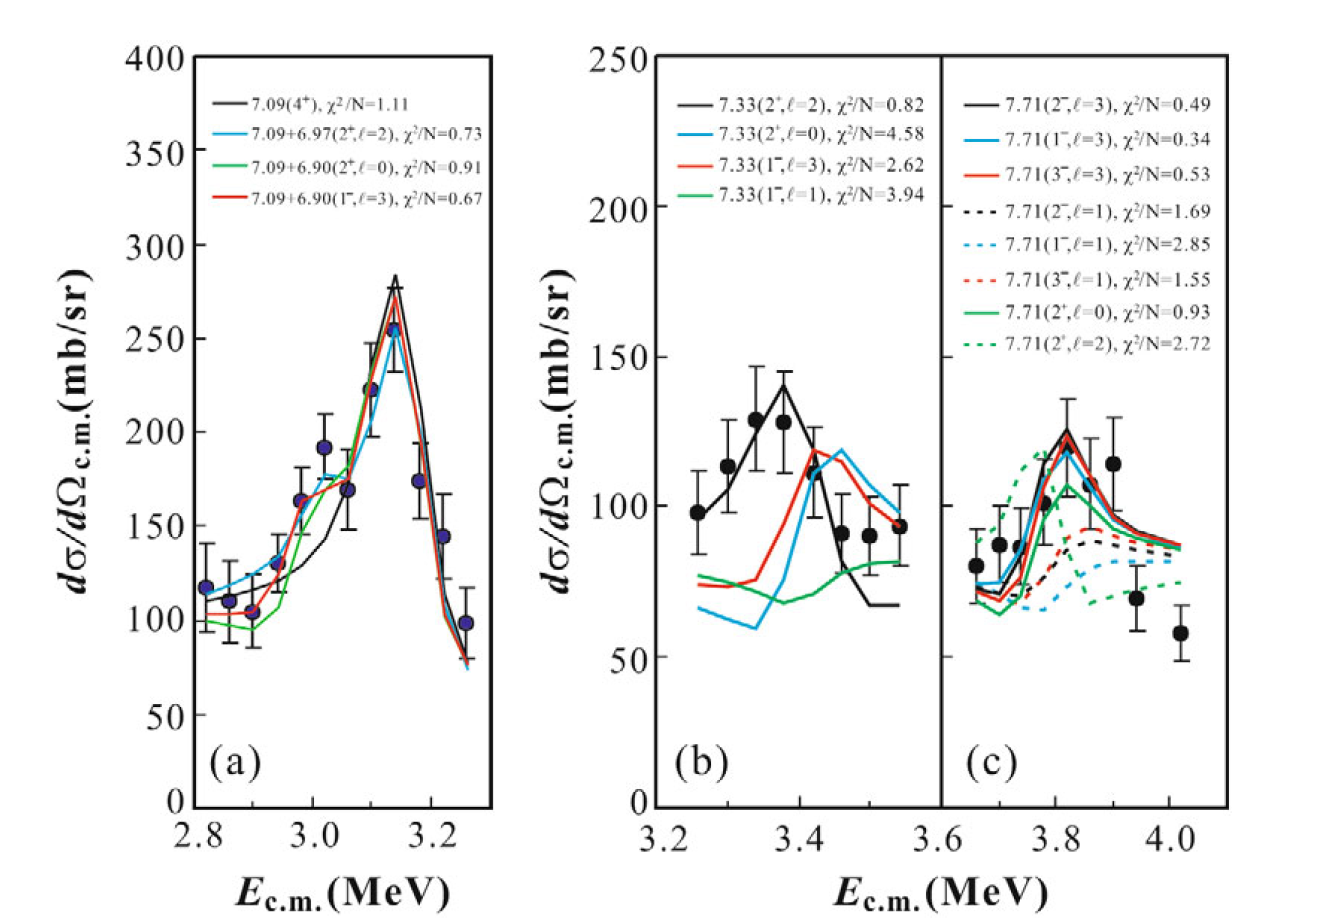
\includegraphics[width=0.5\textwidth]{Razure.png}
\caption{Ajustes para las resonancias aisladas 7.34 y 7.71 MeV y la resonancia doble $7.1$ MeV.}
\label{Fig:11}
\end{figure}


\subsection{Conclusión}

Del estudio realizado por el instituto de física moderna de China en Lanzhou \cite{Astrophysics} en colaboración con otros grupos de investigación chinos a través del experimento anterior y un analisis a través del formalismo R-Matricial nos dice que los estaos excitados del $^{17}$Ne 7.05 MeV ($2^+$)  y 7.12 MeV ($4^+$) contribuyan mas a la reacción nuclear $^{14}$O($\alpha$,p)$^{17}$F que otros estados anteriormente considerados, lo que también incrementa en un factor $\sim$1.2/2 la cantidad de procesos respecto anteriores investigaciones \cite{Astrophysics1} y \cite{Astrophysics2} en la temperatura $\sim$ 2 GK debido a este estado excitado +2. En la tabla \ref{tab:01} vemos los ratio de creación de $^{14}$O($\alpha$,p)$^{17}$F según el experimento anteirormente citado \cite{Astrophysics} y otros anteriores \cite{Astrophysics1},\cite{Astrophysics2} y \cite{Astrophysics3}, y en la imagen \ref{Fig:12} la representación de estos datos. La relación entre la tasa de producción y los datos energías es complicada \cite{Astrophysics} pag.5-6, aunque de manera naif podamos decir que depende de la suma sobre todas las reacciones de una función que depende del espín de la resonancia $J$, de la anchura de la resonancia $\Gamma_\alpha$ y de la energía de resonancia $E_{r}^i$.


\begin{figure}[h!] \centering
	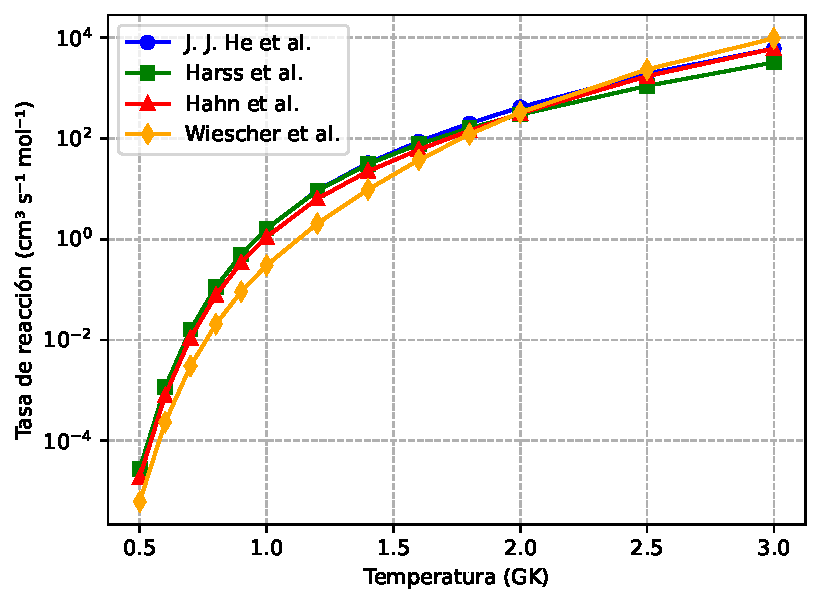
\includegraphics[width=0.5\textwidth]{Final.pdf}
	\caption{Gráfica con los datos de la tabla \ref{tab:01}, reacción  $^{14}$O($\alpha$,p)$^{17}$F.}
	\label{Fig:12}
\end{figure}

\begin{table*}[t]
	\centering
	\caption{Ratio de reacciones $^{14}\text{O}(\alpha, p)^{17}\text{F}$ en unidades de $\text{cm}^3\text{s}^{-1}\text{mol}^{-1}$.}
	\begin{tabular}{c|c|c|c|c}
		\toprule
		$T$ (GK) & {J. J. He et al. \cite{Astrophysics}} & {Harss et al. \cite{Astrophysics1}} & {Hahn et al. \cite{Astrophysics2}} & {Wiescher et al. \cite{Astrophysics3}} \\
		\midrule
		0.5 & 2.75e-5 & 2.75e-5 & 1.89e-5 & 6.14e-6 \\
		0.6 & 1.15e-3 & 1.15e-3 & 7.91e-4 & 2.32e-4 \\
		0.7 & 1.60e-2 & 1.60e-2 & 1.10e-2 & 3.03e-3 \\
		0.8 & 1.12e-1 & 1.12e-1 & 7.70e-2 & 2.05e-2 \\
		0.9 & 4.99e-1 & 4.98e-1 & 3.43e-1 & 9.08e-2 \\
		1.0 & 1.62e+0 & 1.62e+0 & 1.11e+0 & 3.03e-1 \\
		1.2 & 9.32e+0 & 9.19e+0 & 6.38e+0 & 2.04e+0 \\
		1.4 & 3.26e+1 & 3.10e+1 & 2.23e+1 & 9.70e+0 \\
		1.6 & 8.68e+1 & 7.73e+1 & 6.00e+1 & 3.74e+1 \\
		1.8 & 2.00e+2 & 1.60e+2 & 1.43e+2 & 1.21e+2 \\
		2.0 & 4.18e+2 & 2.99e+2 & 3.17e+2 & 3.30e+2 \\
		2.5 & 1.94e+3 & 1.11e+3 & 1.73e+3 & 2.35e+3 \\
		3.0 & 6.11e+3 & 3.25e+3 & 6.12e+3 & 9.77e+3 \\
		\bottomrule
	\end{tabular}
	\label{tab:01}
\end{table*}



%----------------------------------------------------------------------------------------
%	REFERENCE LIST
%----------------------------------------------------------------------------------------


\phantomsection
\bibliographystyle{unsrt}
\bibliography{sample.bib}

%----------------------------------------------------------------------------------------

\end{document}